\documentclass[times, utf8, diplomski]{fer}
\usepackage{booktabs}
\usepackage[croatian]{babel}
\usepackage[utf8]{inputenc}
\usepackage{pdfpages}

\setcounter{secnumdepth}{3}
\setcitestyle{numbers}
\graphicspath{ {./images/} }

\begin{document}

\thesisnumber{1373}

\title{Analiza i usporedba sigurnosnih mehanizama u Internetu stvari}

\author{Filip Ptiček}

\maketitle

% Ispis stranice s napomenom o umetanju izvornika rada. Uklonite naredbu \izvornik ako želite izbaciti tu stranicu.
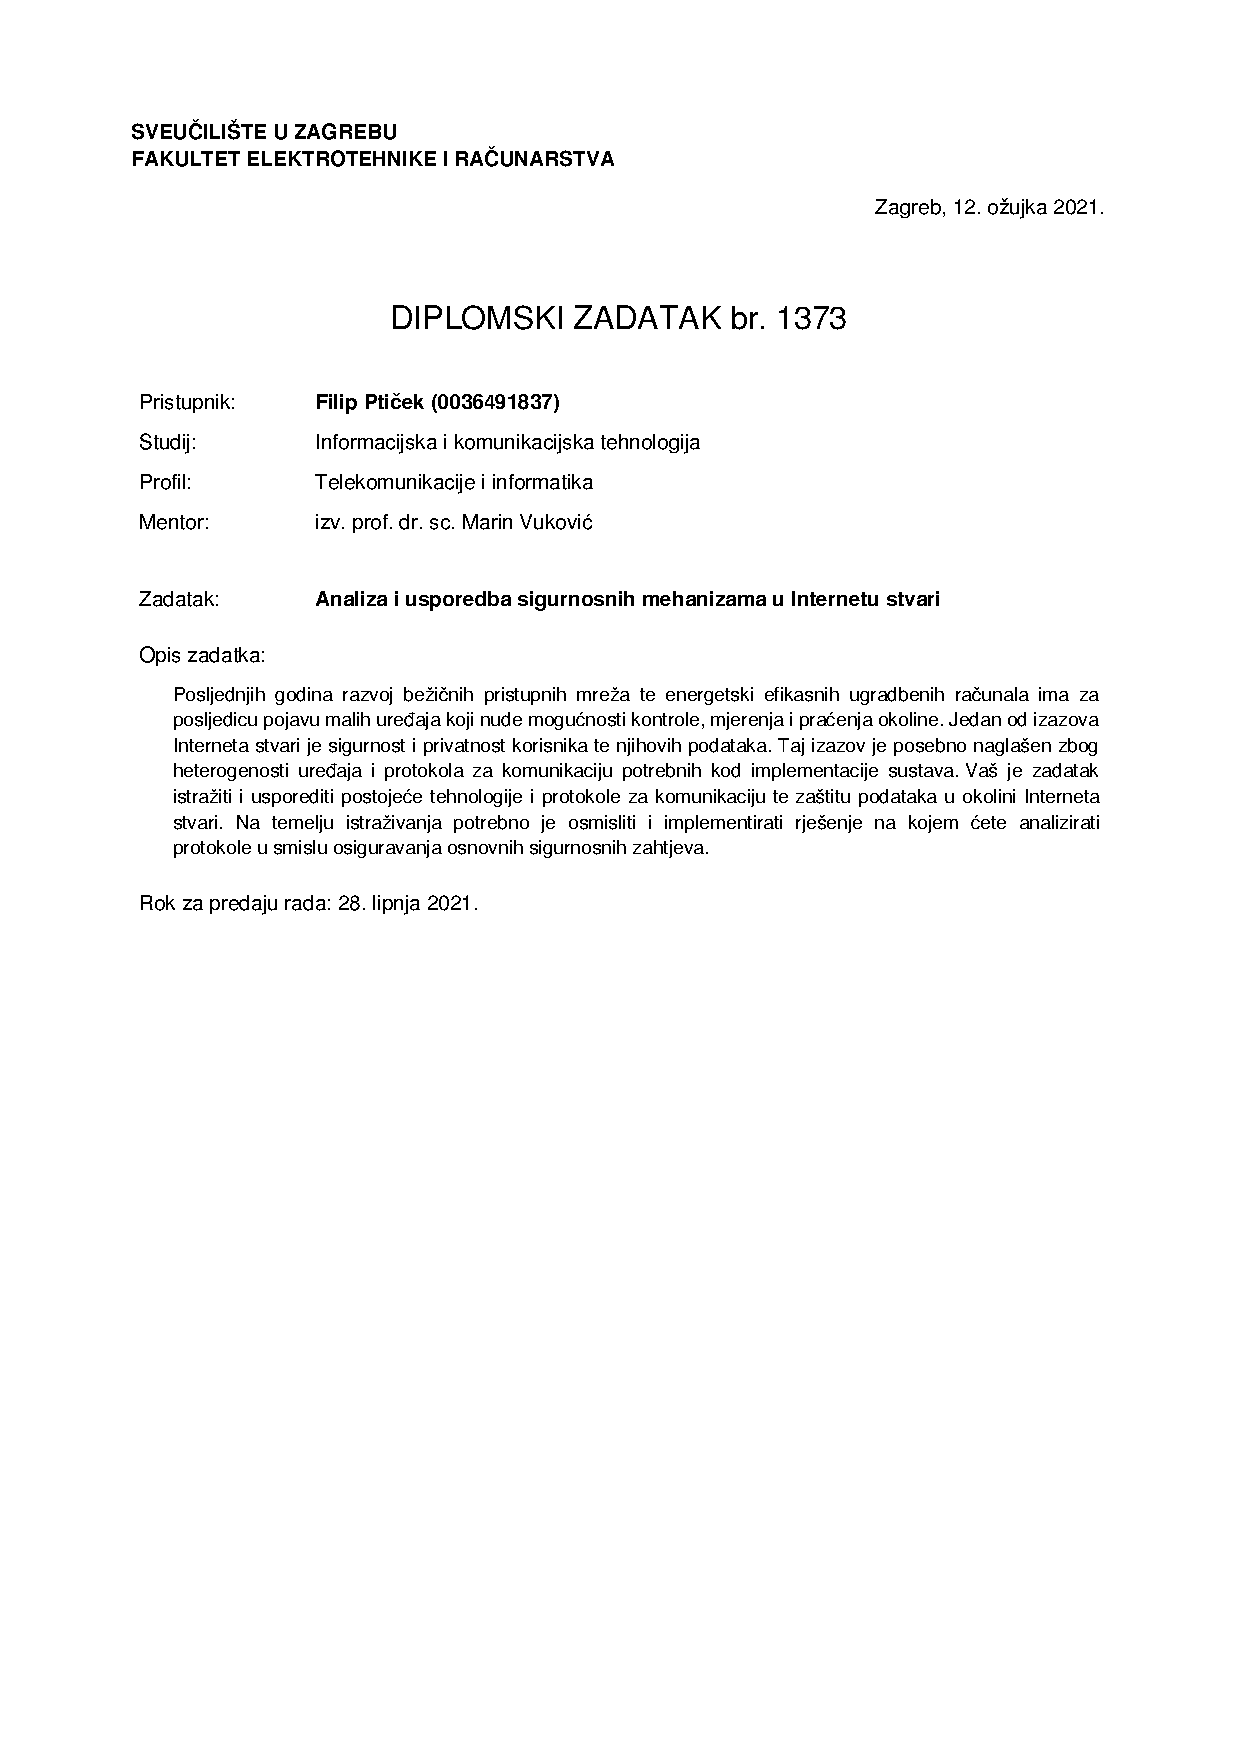
\includepdf[pages=-,fitpaper=true]{zadatak.pdf}

% Dodavanje zahvale ili prazne stranice. Ako ne želite dodati zahvalu, naredbu ostavite radi prazne stranice.
\zahvala{}

\tableofcontents

\chapter{Uvod}
Cola aparat\citep{Coke}

\chapter{Internet stvari}

\section{Definicija}
\emph{The International Telecommunication Union(ITU-T)} je specijalizirana agencija Ujedinjenih Naroda za informacijske i komunikacijske tehnologije. ITU-T definira Internet stvari kao globalnu infrastrukturu za informacijsko društvo, koja omogućava napredne usluge međusobnim povezivanjem (fizičkih i virtualnih) stvari na temelju postojećih i razvijajućih interoperabilnih informacijskih i komunikacijskih tehnologija. Iskorištavanjem identifikacije, prikupljanja podataka, obrade i komunikacijskih sposobnosti, Internet stvari u potpunosti upotrebljava mogućnosti povezanih stvari kako bi ponudio usluge za mnogo različitih primjena, uz osiguravanje sigurnosti i privatnosti. Sa šire perspektive, Internet stvari može biti percipiran kao vizija s tehnološkim i društvenim implikacijama.\citep{ITU-T/IoT} Informacijske i komunikacijske tehnologije (ICT) pruže komunikaciju u bilo koje vrijeme i na bilo kojem mjestu dok Internet stvari dodaje još jednu dimenziju gdje se radi o bilo kojoj stvari u komunikaciji. Te tri dimezije komunikacije su prikazane na sljedećoj slici.
\begin{figure}[htb]
    \centering
    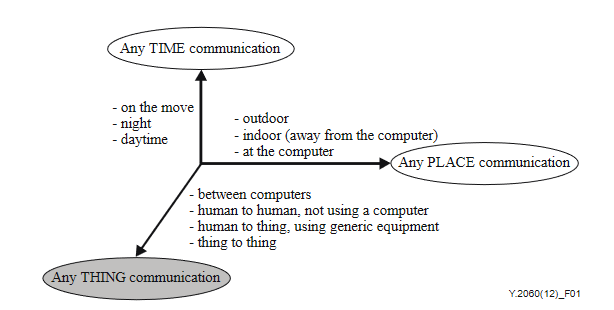
\includegraphics[width=14cm]{images/3dimenzije.png}
    \caption{Nova dimenzija komunikacije predstavljena u Internetu stvari\citep{ITU-T/IoT}}
    \label{fig:3-dim}
\end{figure}

ITU-T također definira pojmove uređaja i stvari u kontekstu Interneta stvari. Uređaj je dio opreme s obaveznom mogučnošću komunikacije i neobaveznim mogućnostima opažanja, aktuacije te prikupljanja, pohrane i obrade podataka. Pojam stvari je definiran kao objekt u fizičkom svijetu (fizička stvar) ili u informacijskom svijetu (virtualna stvar) koja ima sposobnost da bude identificiran i integriran u komunikacijsku mrežu. Fizičke stvari postoje u fizičkom svijetu i imaju sposobnosti biti opažene, aktuirane i povezane, a virtualne stvari potoje u informacijskom svijetu i imaju sposobnosti biti spremljene, obrađene i pristupljene. Neki od primjera fizičkih stvari su: okolina, industrijski roboti, dobra i električna oprema, dok primjeri virtualnih stvari su multimedijski sadržaji i programska podrška.

\section{Referentni model}
Ako promatramo Internet stvari kao jedan zaseban ekosustav potrebno je definirati referentni model prema kojem možemo opisati sve dijelove sustava i njegove zahtijeve. S obzirom na to da je Internet stvari pojam koji opisuje povezanost stvari, a ne i konkretan referentni model, od pojave samog pojma su se predlagali različiti modeli koji bi predstavljali cijeli spektar mogućnosti i zahtijeva Interneta stvari. 
\begin{figure}[htb]
    \centering
    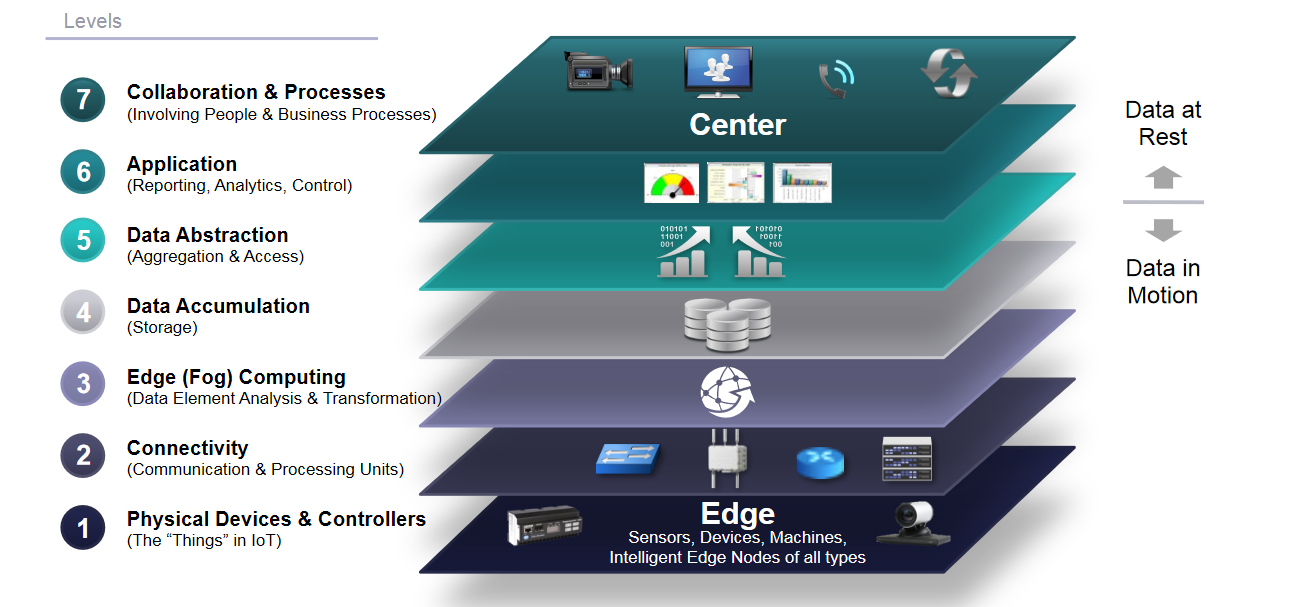
\includegraphics[width=14cm]{images/ciscomodel.png}
    \caption{Cisco Internet stvari referentni model\citep{CiscoIotModel}}
    \label{fig:ciscomodel}
\end{figure}

Ciscov referentni model Interneta stvari\citep{CiscoIotModel} definira višeslojni model od kojih svaki sloj definira terminologiju koja može biti standardizirana kako bi se stvorio globalni referentni okvir. Ovaj model ne definira lokalnost komponenata već opisuje zadatke koje svaki sloj obavlja kako bi se održala jednostavnost, omogućila skalabilnost i osigurala potpora. Model također definira funkcije koje su potrebne kako bi sustav Interneta stvari bio kompletan. Na slici 2.2 je prikazan Ciscov Internet stvari referentni model i njegovi slojevi. Put podataka između slojeva je dvosmjeran, dok put kontrolnih informacija je u s viših slojeva prema nižim slojevima. Kod promatranja je put informacija u obrnutom smjeru, od nižih slojeva prema višim. 

\subsection{Fizički uređaji i kontroleri}
Referentni model počinje s prvim slojem: fizički uređaji i kontroleri koji mogu upravljati s više uređaja. Ovo je sloj koji opisuje stvari u kontekstu Interneta stvari i uključuje različiti raspon uređaja koji šalju i primaju informacije. Uređaji 
su različitih veličina, izgleda i namjene te potječu od različitih proizvođača. Kako bi se pojednostavila kompatibilnost referentni model općenito opisuje razinu obrade potrebne od uređaja. Neke od osnovnih sposobnosti uređaja uključuje: pretvorbu analognih u digitalne signale, generiranje podataka i mogućnost da se uređajem upravlja i šalju upiti.

\subsection{Povezanost}
Komunikacije i povezanost su sarđani u drugom sloju. Najvažnija mogućnost ovog sloja je sposobnost pouzdane i pravovremenog prijenosa informacija. Time se definira prijenos između uređaja i mreže, između mreža te između mreže i računanja na rubu mreže na trećem sloju. Jedan od cilja referentnog modela je da se sva komunikacija odvija putem postojećih mreža. Kako neki uređaji ne podržavaju IP protokol, potrebno je u mrežu uvesti prilaze \engl{gateway} koji će služiti kao posrednik između uređaja i ostatka mreže. Na ovom sloju se pojavljuje velika heterogenost komunikacijskih i pristupnih protokola koji uvelike ovise o željenoj namjeni uređaja prvog sloja. Ovaj sloj je usko povezan sa OSI modelom te sadrži protokole fizičkog, podatkovnog, mrežnog, transportnog, prezentacijskog, aplikacijskog i sloja sesije.

\subsection{Računarstvo na rubu mreže}
Funckija trećeg sloja je vođena potrebom za pretvaranjem mrežnog podatkovnog prometa u informacije koje su prikladne za pohranu podataka i za obradu na višim slojevima. Treći sloj je zadužen za obradu podataka i njihovu transformaciju. Jedno od načela ovog referentnog sloja je da se obrada podataka odvija što je ranije moguće i što bliže rubu mreže kako bi se smanjila potreba za odvijanjem obrade velikog skupa podataka na udaljenom i centralnom mjestu. Obrada na trećem sloju obuhvaća razne primjere poput: evaluacije, formatiranja, proširivanja/dekodiranja, redukcije i procjene značenja podataka.

\subsection{Akumulacija podataka}
Mrežni sustavi su izgrađeni za pouzdani prijenos podataka. Prije četvrtog sloja podaci su u stanju prijenosa. Takvi podaci proizlaze iz prvog i prolaze kroz drugi i treći sloj. Kako u nekim slučajevima ne postoji potreba za trenutnom obradom tih podataka, oni dolaze do četvrtog sloja gdje se podaci spremaju u memoriju. Na ovom sloju su podaci trajni i nepromjenjivi te spremni za posluživanje višim slojevima referentnog modela. Četvrti sloj određuje jesu li podaci važni za više slojeve, ako jesu, potrebno je osigurati načine posluživanja tih podataka zahtijevima viših slojeva. Određuje je li potrebno da podaci budu trajni, tj. treba li podatke spremiti na trajnu ili ih je dovoljno spremiti u radnu memoriju za kratkoročnu upotrebu. Kakav tip pohrane podataka je potreban, datotečni sustav, distribuirani datotečni sustav ili neki oblik baze podataka. Na koji način je organizirano spremanje podataka te je li potrebno podatke spojiti, preračunati i agregirati s prethodno spremljenim podacima. Ukratko, zadaća četvrtog sloja je da podatke bazirane na događajima pretvori u podatke nad kojima se rade upiti za potrebe viših slojeva.

\subsection{Apstrakcija podataka}
Funkcije apstrakcije podataka petog sloja su fokusirane na prikazivanje podataka i njihovu pohranu na način koji dozvoljava razvoj jednostavnijih, brzih aplikacija. Kako u modelu Interneta stvari više uređaja koji generiraju podatke tako postoje različiti razlozi zašto podaci nisu prisutni na istom podatkovnom spremištu: previše podataka za spremanje na jedno mjesto, uređaji su geografski odvojeni, a obrada je opitmizirana lokalno, postoji potreba za različitim načinima obrade podataka te se koriste različiti načini akumulacije podataka. Zbog tih razloga peti sloj je zadužen za različite vrste obrade poput ujednačavanja različitih formata podataka iz različitih izvora, osiguravajući dosljednu semantiku podataka kroz različite izvore, potvrda o potpunosti podataka šestom aplikacijskom sloju, zaštita podataka korištenjem autorizacijskih i autentifikacijskih mehanizama te noramliziranje i indeksiranje podataka za brz pristup od strane aplikacija.

\subsection{Aplikacije}
Na šestom sloju se nalazi aplikacijski sloj koji obavlja interpretaciju informacija. Ovaj referentni model ne definira strogo aplikaciju. Aplikacije se razlikuju na temelju različitih tržišta, prirode podataka i poslovnih potreba. Primjeri različitih potreba su aplikacije koje su usredotočene na promatranje i prikupljenje podataka, neke aplikacije se koriste za kontrolu uređaja dok neke kombiniraju podatke s uređaja i drugih izvora. Aplikacije predstavljaju različite modele upotrebe, razvojnih obrazaca, korištene razvojne programske podrške te krajnje kompleksnosti upotrebe. Neki primjeri aplikacija su povezane sa specijaliziranim industrijskim riješenjima, mobilne aplikacije koje obavljaju jednostavne interakcije, izrada izvješća povezanih uz poslovne procese, analitičke aplikacije koje obrađuju i interpretiraju podatke važne za poslovne odluke i aplikacije za upravljanje i kontroliranje ostatkom sustava. Ako su prijašnji slojevi dizajnirani pravilno to će utjecati na količinu posla koje sama aplikacija mora raditi dok ću to uzvrat olakšati procese na sedmom sloju. 

\subsection{Suradnja i procesi}
Zadnji sedmi sloj referentnog modela uključuje ljude i poslovne procese. Ljudi koriste aplikacije i pridružene podatke za svoje specifične potrebe. Često, više ljudi koriste iste aplikacije za različite svrhe. Tako cilj cijelog sustava Interneta stvari nije sama aplikacija nego kao ispomoć u radu ljudi. Aplikacije pomažu ljudima kako bi mogli obavljati različite poslovne procese uz odgovarajuće podatke u pravo vrijeme. Poslovni procesi nerijetko uključuju rad i komunikaciju između više ljudi. Ljudi surađuju i komuniciraju međusobno kako bi potpora Interneta stvari bila korisna. Zato ti procesi zahtijevaju više koraka koji obuhvaća više aplikacija. Stoga zadnji sloj predstavlja višu razinu od jedne aplikacije.

\section{Izazovi}
Internet stvari kao pojam i skup tehnologija donosi i određene izazove. S obzirom na to da je Internet stvari široko područje koje ima različita područja primjene tako su i izazovi s kojima se kod razvoja, planiranja i održavanja sustava susreče brojni. U nastavku su nabrojani i opisani neki od tih izazova.
%Treba dopisati

\subsection{Heterogenost}
Heterogenost se pojavljuje na svakom implementacijskom koraku Internet stvari sustava. Heterogenost uređaja, komunikacijskih, pristupnih i transportnih protokola, programske podrške i samih potreba korisnika. Naravno ovakva vrsta heterogenosti se javlja zbog različitih potreba i radnim procesa. Uređaji koji su koriste nude različite potrebe u vidu veličine, potrebe za vanjskim napajanjem te dometu komunikacijskih kanala, radilo se o žičanoj ili bežičnoj komunikaciji. Protokoli koji vrše komunikaciju između uređaja i nekog oblika prilaza također ovise o tim potrebama, radilo se o potrebi za velikim transportnim brzinama ili o korištenje radiokomunikacije niske snage kako bi se očuvala energija uređaja. Također treba li komunikacija biti pouzdana i sigurna ovisi o korištenju različitih transportnih protokola te kriptografskih algoritama. Na sve navedeno utječu i sami radni procesi i potrebe korisnika. Ovisno o tome sami sustavi su osmišljeni za potrebe korisnika.

Heterogenost koja se javila u prvim razdobljima razvoja Interneta svari je povezano s nepostojanjem standardizacije i interoperabilnosti uređaja i postojećih programskih platformi. Tako se na primjeru pametnih domova pojavili različiti pametni uređaji od kojih je svaki zahtijevao vlastitu programsku platformu za upravljanje zbog nepostojanja interoperabilnosti s centralnim upravljačkim platformama. Kroz vrijeme su se pojavili zajednički napori prozivođača i različitih standardizacijskih tijela da se ovisno o području primjene Internet stvari sustava postigne standardizacija komunikacijskih protokola i semantike informacija kako bi se postigla bolja interoperabilnost.

\subsection{Raspodijeljenost}
Kako u sustavima Internet stvari sudjeluju različiti uređaji različitih prostornih lokacija tako se javlja i potreba za raspodijeljenosti sustava. Uređaji mogu biti mobilni što uvelike utječe na način pristupa kraljnjih programskih platformi s kojima uređaji komuniciraju. Od dovođenja uređaja u sustava, upravljanja uređaja, promatranja uređaja i samih aplikacija preko kojih se ti postupci provode se odvijaju raspodijeljenim putem. U nekim sustavima broj sudionika dostiže veliku brojku te je kod takvih sustava važno da se paralelno i konkurentno mogu odvajati aktivnosti. Otpornost na kvar je još jedan od zahtijeva koji prati raspodijeljene sustave kako bi se omogućo nesmetan rad sustava. Kod ispada i kvarova posljedice koje sustav Interneta stvari može imati na vanjski svijet je velik. Pogotovo u primjerima gdje se nadzire neki kritični sustavi poput industrijskih postrojenja. Također u pametnim domovima gdje različiti kučanski aparati su pretvoreni u pametne uređaje, kvarom poslužitelja mogu postati neupotrebljivi te je važno da postoji redudantnost servisa s kojima uređaji komuniciraju.

\subsection{Sigurnost}
Sigurnost informacija i samih sustava je važan aspekt Interneta stvari u kojem sve više uređaja oko nas postaje umreženo. Problemi koji se javljaju su povezani s pokušajem brzog razvoja riješenja zbog konkurentnosti na tržištu, stavljanje u prvobitni plan funkcionalnosti sustava te dostupnosti prema korisnicima što stavlja sigurnost tih sustava u drugi plan. Kako mnogi uređaji i cjelokupni sustavi uvelike imaju kritične zadatke, poput medicinskih uređaja ili automobila, kompromitacija istih zbog sigurnosnih propusta može imati negativne posljedice. Također neki od primjera napada na sustave nije kako bi se napravila šteta sustavu već za iskorištavanje procesne snage sustava u botnetovima. Sigurnosni propusti se mogu poajviti na svakom dijelu sustava od uređaja, komunikacijskih kanala, poslužitelja, baza podataka i korisničkih sučelja sustavima. Neki od najvažnijih sigurnosnih zahtijeva na koje treba obratiti pozornost tijekom razvoja sustva Internet stvari je obrađeno u trećem poglavlju.

\subsection{Privatnost}
Privatnost je uz sigurnost izazov s kojim se susreću mnogi sustavi Interneta stvari. Pametni uređaji koji se nalaze u našoj blizini imaju mogućnosti pratiti i bilježiti podatke o nama i našoj okolini. Kako korisnici priključuju sve više i više uređaja to je količina prikupljenih podataka veća čime i povreda privatnosti može imati negativne posljedice na korisnika. Povrede te privatnosti mogu dolaziti u različtim oblicima. Od osobnih informacija koje mogu detaljno identificirati korisnika daju mogućnost napada u obliku krađe identiteta, medicinskih podataka ili pristupnih lozinki različitim servisima do kompromitacije sigurnosnih kamera što dozvoljava napadačima izravno pračenje korisnika. Privatnost podataka koji nisu isključivo vezani uz krajnje korisnike su i podaci pravnih osoba gdje može doći do narušavanja poslovnih tajni, autentifikacijskih i autorizacijskih podataka za razne servise i sigurnosne sustave. Kako pristupiti zaštiti privatnosti je usko povezano sa sigurnošću sustava te je obrađeno u trećem poglavlju.

\subsection{Integracija}
Nove tehnologije donose i nove integracijske probleme sa sobom. U slučaju Interneta stvari ovaj izazov veći zbog heterogenosti svih dijelova koji čine sustave. U slučaju heterogenosti sloja podatkovne poveznice i količine različitih protokola koji se koriste postoji problem uvođenja novih prijamnika i prilaza za te uređaje. Radi li se o niskofrekventnim riješenjima poput NFC-a ili protokolima poput ZigBee postoji potreba korištenja posebnih čitaća ili prijamnika dok se taj problem ne pojavljuje kod WiFi protokola čija pristupna točka već postoji u većini domova. Nakon toga dolazimo do komunikacijske integracije između uređaja i poslužitelja, tj. programskih platformi. Na koji način će se odvijati prijenos podatka, kako će ti podaci biti organizirani te semantičko značenje tih istih podataka. Početkom razvoja riješenja Internet stvari prvobitno su svi sustavi imali vlastite pristupne aplikacije. S pojavom želje za automatizacijom i međusobnom komunikacijom između uređaja različitih proizvođača počele su se razvijati platforme koje omogućuju interoperabilnost među sustavima te mogućnost upravljanja i praćenja uređaja putem jedne pristupne aplikacije. Kroz razvoj tih platformi proizvođači su počeli integrirati nove i postojeće uređaje da budu kompatibilni s njima.

\section{Područja primjene}
Internet stvari je široko u svojem području primjena. U današnjem svijetu postaje sve prisutnije u svakom aspektu života ljudi i taj trend će se nastaviti. Od naših domova do industrijskih postrojenja Internet stvari omogućava pojednostavljenje naših života i posolvnih procesa. U nastavku su navedeni neke od glavnih područja primjene Interneta stvari i riješenja koja se koriste u tim područjima:
\begin{itemize}
    \item Pametni dom
    \begin{itemize}
        \item Pametna rasvjeta
        \item Pametni kučanski aparati
        \item Detekcija uljeza
        \item Upravljanje energijom
    \end{itemize}
    \item Pametni grad
    \begin{itemize}
        \item Pametni parking
        \item Upravljanje otpadom
        \item Pametna rasvjeta
        \item Reagiranje na hitne slučajeve
    \end{itemize}
    \item Okoliš
    \begin{itemize}
        \item Praćanje vremena
        \item Praćenje zagađenja zraka
        \item Praćenje zagađenja bukom
        \item Detekcija požara
    \end{itemize}
    \item Prodaja
    \begin{itemize}
        \item Upravljanje inventarom
        \item Pametni automati za prodaju
        \item Pametne blagajne
        \item Pametno plaćanje
    \end{itemize}
    \item Logistika
    \begin{itemize}
        \item Praćenje flote vozila
        \item Praćenje pošiljaka
        \item Dijagnostika vozila na daljinu
        \item Generacija i vremensko raspoređivanje voznih ruta
    \end{itemize}
    \item Industrija
    \begin{itemize}
        \item Dijagnostika strojeva
        \item Praćenje dijelova proizvodnje
        \item Automatizacija procesa
    \end{itemize}
    \item Poljoprivreda
    \begin{itemize}
        \item Pametno navodnjavanje
        \item Praćenje usjeva
        \item Automatizacija obrađivanja
    \end{itemize}
\end{itemize}

\section{Trendovi}
Internet svari se pojavio kao zamisao za daljnju budućnost, ali je već danas sadašnjost u socijalnim i proizvođačkim aspektima svijeta. Broj umreženih uređaja raste što je prikazano na sljedećoj slici. %doradi ovaj dio
\begin{figure}[htb]
    \centering
    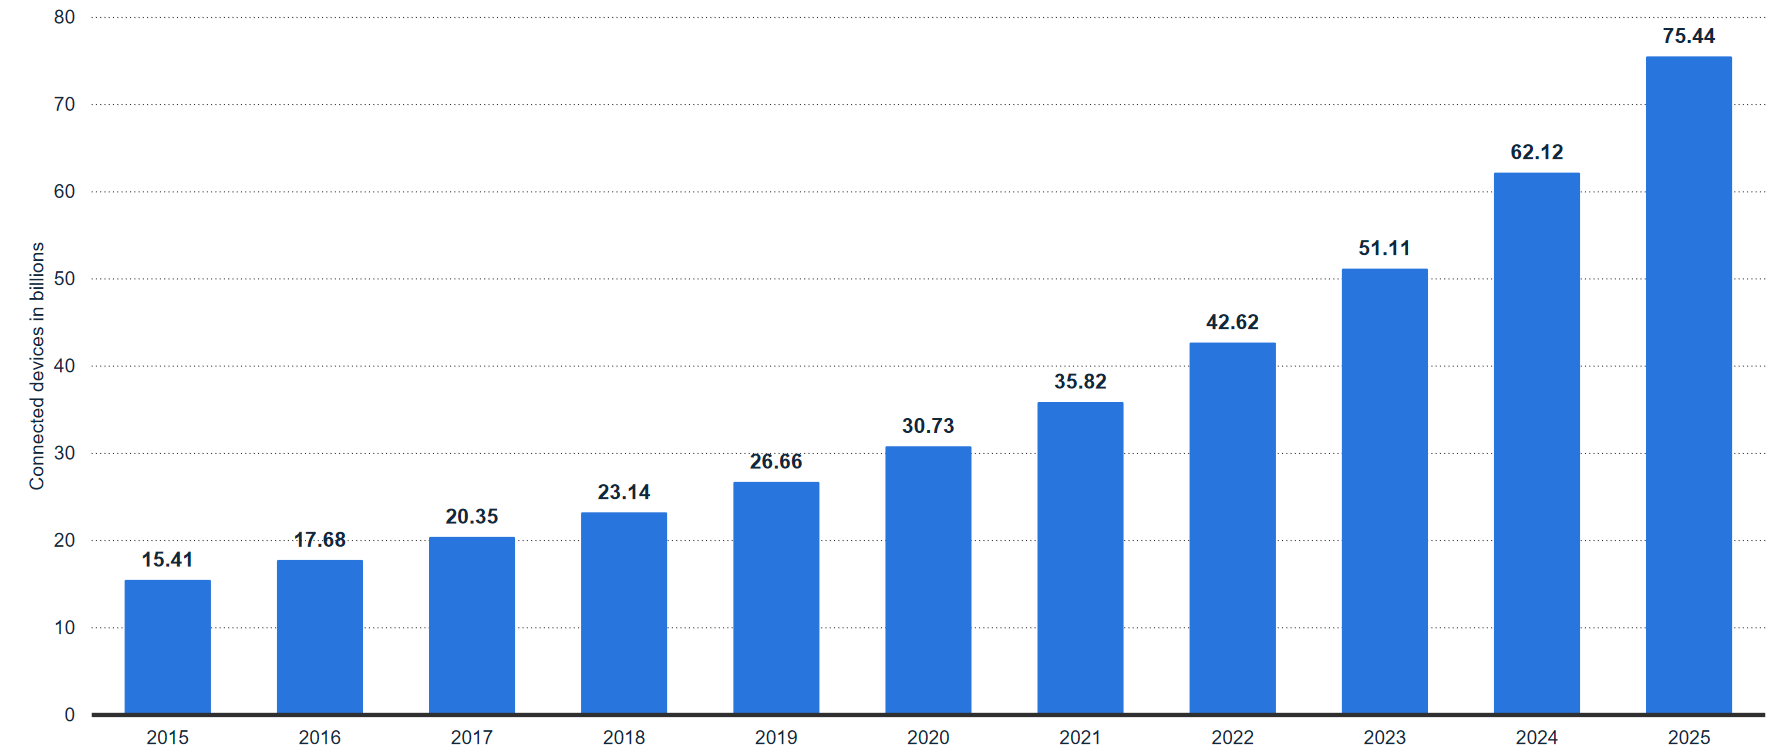
\includegraphics[width=16cm]{images/number-of-installed-iot.png}
    \caption{Broj povezanih Internet stvari uređaja\citep{IotNumber}}
    \label{fig:iotdevices}
\end{figure}

%Add stuff

\chapter{Sigurnosni zahtijevi u Internetu stvari}

\section{OWASP Top 10}
The Open Web Application Security Project® (OWASP) je neprofitna organizacija čiji je cilj napredak i poboljšanje računalne sigurnosti informacijskih sustava. OWASP kroz svoje projekte otvorenog koda vođenih putem razvojne zajednice radi na poboljšanju sigurnosti Interneta.

\emph{OWASP Internet of Things Project} je projekt osmišljen kako bi pomogao proizvođačima, programerima i potrošačima bolji uvid i razumijevanje u sigurnosne probleme vezane uz Internet stvari. Na taj način korisnici u bilo kojem dijelu razvojnog procesa mogu donositi bolje odluke kod razvoja, postavljanja i pristupanja tehnologijama Interneta stvari.\citep{owasp1} 2018. godine izlazi \emph{OWASP IoT Top 10} lista koja reprezentira deset najčešćih ranjivosti Internet stvari sustava. Svih deset sigurnosnih ranjivosti su navedeni u nastavku uz opis sigurnosnih zahtijeva koji bi trebali spriječiti te ranjivosti i sigurnosne propuste. 

\subsection{Slabe, pogodljive ili tvrdo kodirane lozinke}
Prvi navedeni sigurnosni problemi kod Internet stvari sustava su vezni uz lozinke. Kako bi se uređaju moglo pristupiti i naknadno ga konfigurirati, uređaji dolaze s korisničkim računima koji služe korisnicima kako bi ih mogli upariti sa željenim sustavim ili kako bi proizvođač mogao upravljati uređajem u slučaju pomoći korisnicima ili ažuriranja uređaja. Za pristup tom korisničkom računu uređaja je potrebna lozinka koju krajnji korisnik kod prve upotrebe treba postaviti. Navike korisnika su većinom da iskoriste njima dobro poznatu lozinku koju koriste i za svoje druge korisničke račune. Ako napadač dobije pristup jednoj njihovoj lozinci ima i pristup ostalim računima. Na taj način se pristup korištenim uređajima koji imaju isto korisničko ime ili e-mail adresu i lozinku uvelike olakšava. Korisnici imaju i naviku koristiti slabe lozinke koje su vrlo česte i jako lako pamtljive. Tako su neke od najčešće korištenih lozinka jednostavni nizovi numeričkih znakova ili nizovi znakova na tipkovnici poput: 123456, 123456789, qwerty, ili sam engleski prijevod lozinke \engl{password}.\citep{pass1}. Napadi na lozinke se provode putem takozvanih \emph{brute force} napada. Kako je procesna snaga današnjih računala dosegla vrlo visoke brzine računanja, tako se jednostavne i kratke lozinke mogu pogoditi u vrlo kratkom vremenu.

Ovakvi propusti ne zaobilaze ni proizvođače samih sustava i uređaja. Kod proizvodnje proizvođači na uređaje postavljaju iste lozinke za sve uređaje kako bi kod testiranja ispravnosti lakše pristupili istima. Jedan od najboljih pokazatelja takvog pristupa su usmjerivači/modemi telekom operatera za pristup Internetu koji imaju postavljenu istu zadanu lozinku i korisničko ime poput "admin" ili "user" koju krajnji korisnici uređaja nikada ne promjene. Problem se također pojavljuje i u tvrdo kodiranim \engl{hard coded} lozinkama. Proizvođači postave takve lozinke na uređaje kako bi se uređaji mogli nesmetano povezati s vanjskim servisima, kako bi se proizvođači povezli na uređaj zbog otklanjanja pogrešaka ili kao način za vanjsko upravljanje uređaja. Ako napadač ima fizički pristup uređaju on može skenirati memoriju i pomoću raznih alata pronači lozinku spremljenu na samom uređaju. A kako prozivođači najvjerojatnije koriste istu lozinku za sve iste modele uređaja, napadač ima lak način za pristup i ostalim istim uređajima.

Kako bi se spriječila ova vrsta ranjivosti neki od sigurnosnih zahtijeva koji bi se trebali pratiti su sljedeći. Korisnici bi kod prve upotrebe uređaja trebali promjeniti zadanu lozinku koristeći duge, kompleksne i jedinstvene nizove znakova. Najjednostavniji način postići te zahtijeve je korištenjem upravitelja lozinkama. Oni daju mogućnost generiranja lozinki uz mogućnost spremanja istih bez potrebe da korisnik mora pamtiti sve jedinstvene i duge lozinke. Što se tiče zahtijeva sa strane prozivođača, oni bi trebali razriješiti bolje načine upravljanja uređajima kako bi se izbjeglo korištenje istih ili čak tvrdo kodiranih lozinka za pristup uređaju ili vanjskim servisima. Također bi proizvođači trebali upozoriti korisnika kod uspostave uređaja da promijeni zadanu lozinku.

\subsection{Nesigurne mrežne usluge}
Internet stvari uređaji koriste razne mrežne usluge kako bi mogli komunicirati s vanjskim servisima. Kako je moguće pristupiti tim uređajima putem Interneta potrebno je pravilno osigurati sigurnost tih mrežnih usluga koje se izvršavaju. Neautoriziran pristup preko usluga iskorištavajući zadane lozinke, otvorene mrežne priključke te nepravilno podešeni vatrozidi dozvoljavaju napadaču da dobije pristup uređajima i poslužiteljima. Takvi napadi dozvoljavaju izvršavanje malicioznog koda, iskorištavanje uređaja za botnet, krađu podataka ili onesposobljavanje sustava.
%Expand a little bit

Neki od sigurnosnih mjera koje se mogu poduzeti za osiguravanje mrežnih usluga su: \begin{itemize}
    \item korištenje zasebne lokalne mreže za sve pametne uređaje,
    \item spajati uređaje na isključivo sigurne mreže,
    \item instaliranje regularnih softverskih ažuriranja,
    \item isključivanje svih usluga koje pružaju vanjski pristup uređaju,
    \item isključivanje nepotrebnih mrežnih priključaka i usluga,
    \item isključivo korištenje protokola koji koriste enkripciju.
\end{itemize}

\subsection{Nesigurna sučelja ekosustava}
Nesigurna web sučelja, pozadinski API-jevi, servisi u oblaku i mobilna sučelja, koja dozvoljavaju komunikaciju i interakciju s uređajem, čine sveukupni ekosustav Internet stvari. Kompromitacija bilo kojeg dijela sustava može uzrokovati i kompromitaciju cijelokupnog sustava. Ranjivost kod načina autorizacije i autentifikacije između uređaja i poslužitelja ili korisnika mobilnih i web aplikacija i poslužitelja su jedan od vektora napada na sustav. Također nedostatak ili korištenje slabe enkripcije kod komunikacije može uzrokovati da napadač presretne i iskoristi sakupljene informacije za napad. Nedostatak pravilnog filtriranja ulazno/izlaznih podataka može dovesti do napada poput SQL injekcije. Još jedan projekt OWASP organizacije je \emph{OWASP Top 10 Web Application Security Risks} koji nudi popis najčešćih ranjivosti za web i mobilne aplikacije. Nesigurna sučelja ekosustava imaju direktnu poveznicu s tim ranjivostima koje su: \begin{itemize}
    \item injekcije (SQL, NoSQL, OS, LDAP),
    \item neispravna autentifikacija,
    \item izlaganje osjetljivih podataka,
    \item XML External Entities(XXE) napadi,
    \item neispravna autorizacijska kontrola,
    \item pogrešna konfiguracija servisa,
    \item Cross-Site Scripting(XSS),
    \item nesigurna deserijalizacija podataka,
    \item korištenje bibilioteka i komponenta s poznatim sigurnosnim ranjivostima,
    \item nedovoljno korištenje logova i praćenja sustava.\citep{owasp2}
\end{itemize}

Pravilno podešavanje autorizacije i autentifikacije korisnika, ali i uređaja je najvažniji način osiguravanja raznih sučelja ekosustava. Filtriranje ulaznih i izlaznih podataka spriječava napade injekcijom, pravilno podešavanje poslužitelja da koriste pravilne enkripcijske načine komunikacije dozvoljavaju privatnu i sigurnu komunikaciju. Kroz cijeli ekosustav je potrebno i uspostava logiranja i praćenja sustava kako bi se na vrijeme otkrili nepravilna ponašanja unutar samog sustava.

\subsection{Nedostatak mehanizama za sigurnosna ažuriranja}
Kroz vrijeme, za programska rješenja koja se trenutno koriste na uređaju će se pronači ranjivosti. Kako bi se na vrijeme i jednostavnim putem mogli spriječiti napadi koji iskorištavaju te ranjivosti potrebna su nam softverska ažuriranja, kao i ažuriranja samog ugrađenog programa \engl{firmware} uređaja. Ako ne postoji način kojim dovodimo takva sigurnosna ažuriranja na uređaj postoji rizik za kompromitacijom uređaja. Također ako su i implementirani načini sigurnosnih ažuriranja, potrebno je pridodati pažnju na način te implementacije ažuriranja. Ako se ne provjeravaju digitalni potpisi izvora ažuriranja, moguće je na uređaj poslati maliciozno ažuriranje koje će kompromitirati uređaj. Potrebno je i koristiti sigurne načine prijenosa tih ažuriranja poput enkripcije upotrebljavanog komunikacijskog kanala. 

Trenutnim trendom brzog razvoja novih uređaja, prozivođači često ne daju dovoljno dugi period sigurnosnih ažuriranja. Tako će se desiti da proizvod nakon manje od dvije godine prestane dobivati ažuriranja te će pasti odluka na korisnika o tome hoće li kupiti novi uređaj ili riskirati kompromitaciju istog. Najbolji pokazatelj toga su pametni telefoni od kojih većina tijekom svog perioda upotrebe dobije samo nekoliko sigurnosnih ažuriranja prije nego bude depricirana od strane prozivođača.

Kako bi se uređaji zaštili od budućih napada zbog novootkrivenih sigrunosnih propusta potrebno je pružati korisnicima uređaja nuditi dugotrajna i česta sigurnosna ažuriranja. Prijenos ažuriranja je neophodno prenositi putem sigurnih komunikacijskih kanal koji su enkriptirani. Ažuriranjima koja su dostigla na uređaj je potrebno validirati izvor, provjeriti odgovara li digitalni potpis izvoru od kojeg bi trebalo stići ažuriranje. Također je potrebno i validirati samo ažuriranje kako bi se izbjeglo moguće umetanje malicioznog koda.

\subsection{Upotreba nesigurnih ili zastarijelih komponenti}
Nadovezano na nedostatak mehanizama za sigurnosno ažuriranje, peta po redu od sigurnosnih propusta je upotreba nesigurnih ili zastarijelih komponenti. Mnogi sustavi Internet stvari kao dio svojeg programskog riješenja sadrže otvoreni kod koji održava zajednica koja nije direktno povezana s proizvođačem. Kada se otkrije ranjivost na nekom od korištenih otvorenih rješenja proizvođač ili čeka na sigurnosnu zakrpu, ili u najboljem slučaju će sam riješiti sigurnosni propust te ga javno objaviti kako bi doprinjeo razvoju otvorenog rješenja. Nakon što sigurnosna zakrpa bude razvijena potrebno je ažurirati sve uređaje ili dijelove sustava koji su ugroženi od tog sigurnosnog propust. 

Ako govorimo o Internetu stvari u proizvođačkoj industriji, takozvanoj Industriji 4.0, upotreba zastarijele programske podrške, koja je potrebna zbog jako specifičnih uređaja za prozivodnju, čija zadnja verzija zna datirati i više od deset godina nije rijetka. Uvođenjem takvih uređaja u sustave Interneta stvari također utječe na sigurnost i integritet cijelokupnog sustava te ugrožavanje jednog uređaja može dovesti do napada na cijelog lanca opskrbe. Kod upotrebe gotovih proizvoda poput senzora, videokamera ili pametne rasvijete te integracijom istih u postojeći sustav također treba obratiti pozornost na dostupnost sigurnosnih ažuriranja te stanje uređaja poput je li proizvođač još uvijek nudi sigurnosnu podršku.

Kod planiranja razvoja Internet stvari sustava potrebno je uzeti u obzir trenutno, a i buduće stanje razvojne i sigurnosne podrške vanjske programske potpore i komponenti sustava. Najbolji način za spriječavanje sigurnosnih propusta je korištenje vlastito razvijene programske potpore ili korištenje dobro podržanih vanjskih biblioteka otvorenog koda s jakom i aktivnom razvojnom zajednicom. Uporeba zastarijelih uređaja bez sigurnosne podrške proizvođača ili potporom koja uskoro dotiže krajnji period \engl{end of life} je potrebno izbjegavati. Nakon puštanja sustava u produkciju nadziranje i praćenje vijesti vezanih uz sigurnosne propuste upotrebljenih komponenti i programske podrške je važno kako bi se na vrijeme moglo spriječiti kompromitacija sustava. Sve ovo nije moguće ako bilo koji dio ustava nema implementirane mehanizme za sigurnosna ažuriranja. Ako neka od komponenti dostigne svoj krajnjio period ažuriranja potrebno je tu komponentu ukloniti i zamijeniti ju drugom čija sigurnosna ažuriranja još uvijek su podržana.  

\subsection{Nedovoljna zaštita privatnosti}
Uloga Interneta stvari je djelom prikupljanje različitih podataka i mjerenja. Neki od tih podataka su osobne prirode za korisnika poput: medicinskih podataka ili zvukovnih i video zapisa. Kompromitacija takvih privatnih podataka može negativno utjecati na sigurnost korisnika. Prostor na kojem se privatnost korisnika može narušiti je od samog uređaja koji prikuplja podatke, do komunikacijskih kanala preko kojih se podaci šalju do samih krajnjih servisa koji primaju i obrađuju te podatke, a zatim ih spremaju u baze podataka na poslužiteljma. Nedovoljna zaštita privatnosti je zapravo rezultat svih ostalih nabrojanih sigurnosnih ranjivosti nabrojanih u ovom odjeljku. 

Za očuvanje privatnosti korisnika i načine obrade podataka korisnika u Europskoj uniji postoji uredba donešena od strane Europske unije pod nazivom \emph{Opća uredba o zaštiti podataka(GDPR) (EU) 2016/679}\citep{GDPR}. Cilj uredbe je omogućiti građanima Europske unije veću kontrolu i uvid u podatke koji se prikupljaju. Na taj način građani mogu tražiti brisanje svojih podataka i povećava se odgovornost pravnih osoba koje te podatke prikupljaju. Odgovornost se postiže mogućim nametnutim sankcijama, ako se utvrdi povreda podataka građana. Prikupljanje podataka je moguće uz izrazitu privolu građana korisnika čime se zabranjuje bilo kakvo prikupljanje podataka bez pristanka. 

Enkripcija komunikacijskih kanal nekada ne osigurava i privatnost korisnika. Kako bi pametni uređaji mogli komunicirati s krajnjim poslužiteljima, koji mogu mijenjati svoju odredišnu adresu, koriste se domenska imena. Za razlučivanje tih adresa u brojčanje IP adrese koristi se protokol DNS\engl{Domain Name System}. Kada uređaji rade DNS upite u sadržaju upita se prikazuje i domena upita u nekriptiranom formatu. Na taj način napadač može iz konteksta upita zaključiti koji uređaji proizvođača se nalaze u mreži korisnika. Za neke uređaje je moguće zaključiti i sam tip, a ne samo proizvođač. U sljedećoj tablici možemo vidjeti uređaje i DNS upite koje proizvode:
\begin{table}[h]
    \centering
    \begin{tabular}{| c | c |} 
    \hline
    \textbf{Uređaj} & \textbf{DNS upiti} \\
    \hline\hline
    Nest Security Camera & nexus.dropcam.com \\
     & oculus519-vir.dropcam.com \\
     & pool.ntp.org \\
    \hline
    Amazon Echo & ash2-accesspoint-a92.ap.spotify.com \\ 
     & audio-ec.spotify.com \\ 
     & device-metrics-us.amazon.com \\ 
     & ntp.amazon.com \\ 
     & pindorama.amazon.com \\ 
     & softwareupdates.amazon.com \\
    \hline
    \end{tabular}
    \caption{Primjer DNS upita napravljenih od strane uređaja \citep{Apthorpe2017May}}
    \label{tab:confusion}
\end{table} \\
Još jedan način na koji se može zaključiti o trenutnoj aktivnosti korisnika u vlastitoj mreži je i broj paketa koji se šalje u danom trenutku van mreže i njihova periodičnost. Ako se radi o uređaju koji ima mogućnosti virtualnog asistenta moguće je imati uvid u to kada je korisnik imao interakciju s uređajem. Također kod uređaja koji prate spavanje korisnika se broj razmijenjenih paketa drastično poveća kada korisnik spava.\citep{Apthorpe2017May}

Kako najbolje očuvati privatnost korisnika je pitanje s kojim još uvijek mnogi prozivođači imaju problema. To se očituje u ostalim navedenim sigurnosnim propustima u ovom odjeljku. Zakonskim regulativama postiže se veća svijest o bitnosti zaštite podataka te se samim time proizvođači tjeraju na bolje prakse za očuvanjem podataka. Neki od osnovnih načina zaštite korisničkih podataka su: 
\begin{itemize}
    \item enkripcija podataka u svakom aspektu sustava,
    \item prikupljanje samo nužnih podataka,
    \item anonimiziranje korisnika,
    \item bolja kontrola i uvid u podatke za korisnike.
\end{itemize}

\subsection{Nesigurni prijenos i pohrana podataka}
Podaci koji nisu kriptirani moguće je vrlo lako iščitati. Kriptografijom se postiže sigurnost i privatnost podataka. Kako bi se to postiglo podatke je potrebno kriptirati u svokm koraku njihova nastajanja, prijenosa, obrade i spremanja. Korištenje samih kriptografskih alogritama ne rezultira uvijek i zaštitom podataka. Neki kriptografski algoritmi koriste ključeve nedovoljne dužine i kao takve je potrebno malo vremena da se dešifriraju. Najveći sigurnosni propusti u nedavnoj povijesti povezani su dirketno s nedovoljnim kriptografskim algoritmima ili općenitim nedostatkom šifriranja čime su ugroženi osobni podaci i lozinke korisnika.\citep{DataBreaches} Pozornost se treba posvetiti i kontroli pristupa podacima kako neautorizirani korisnici ne bi mogli pristupiti nedozvoljenim podacima. 

Osnovni sigurnosni zahtijevi koji bi se trebali osigurati su: \begin{itemize}
    \item šifriranje podataka,
    \item pravilno korištenje PKI-a \engl{public key infrastructure},
    \item kontrola pristupa podacima,
    \item korištenje sigurnih protokola za prijenos podataka,
    \item provjera korištenih kriptografskih algoritama za ranjivosti,
    \item korištenje dugih kriptografskih ključeva.
\end{itemize}     

\subsection{Nedostatak mogućnosti upravljanja uređajima}
Nemogućnošću upravljanja uređajima ima posljedicu da uređaji u slučaju otkrivenih sigurnosnih propusta ne mogu biti ažurirani, da uređaje nije moguće na jednostavan način otkloniti i uvesti u ekosustav te naknadno proširivati njihove mogućnosti. Zato je jedan od najvažnijih sigurnosnih zadataka u Internetu stvari ekosustavima upravljanje uređajima kroz njihov životni ciklus. Ako neautorizirani uređaji budu uvedeni u ekosustav, imat će mogućnost dobivanja pristupa ostalim komponentama ekosustava te nadgledanja mreže i presretanja prometa i informacija. 

Zbog heterogenosti trenutnih implementacijskih riješenja jedinstven način upravljanja uređaja je također jedan od problema koji se pojavljuju. Ako imamo više uređaja od kojih svaki zahtijeva svoju platformu i drugačiji način upravljanja, stvara se problem da neki uređaji koji ne zahtijevaju konstantnu pozornost ostanu zaboravljanji te nenadzirani i neažurirani. 

Potrebno je imati implementirane načine upravljanja, nadzora i ažuriranja uređaja prisutnih u sustavu. Otkrivanje i identifikacija uređaja je bitan korak u nadgledanju i zaštiti cijelog ekosustava. Heterogenost implementacijskih riješenja uređaja je još uvijek problem s kojim se integratori riješenja susreću, ali kako cijelo područje sazrijeva dolazimo do različitih platformi koje nude integraciju njih svih u jedinstveni ekosustav. Stoga je kod planiranja sustava potrebno uzeti u obzir uređaje kojim je moguće jedinstveno upravljati kako bi se izbjeglo zanemarivanje uređaja.

\subsection{Nesigurne zadane postavke}
Zadane postavke na pametnim uređajima povezane su uz nekoliko primjera. Takav propust se može očitovati kod univerzalnih zadanih lozinka, tvrdo kodiranim lozinkama ili zadanih postavka programske podrške uređaja. Univerzalne zadane lozinke se pojavljuju kao najednostavniji način prvobitnom pristupu uređaju umjesto nekog drugog načina uspostave uređaja. Takav pristup se mora spriječiti navođenjem upozorenja ili obaveznim postupkom promjene lozinke kod prvobitnog postavljanja uređaja. Tvrdo kodirane lozinke za pristup uređajima je problem koji kod fizičkog ili vanjskog pristupa uređaju može lako dovesti do kompromitacije cijelog sustava te je korištenje takvih lozinka i načina pristupa potrebno izbjegavati. Zadane postavke programske podrške koje mogu dovesti do sigurnosnih propusta je dužnost proizvođača da tijekom testiranja i sigurnosne revizije uoći i onemogući sve nepotrebne i potencijalno nesigurne postavke programske podrške uređaja. To uključuje i sve metode koje su se koristile za testiranje i otklanjanje pogrešaka tijekom razvoja uređaja.

Ovaj sigurnosni propust nije isključivo vezan uz uređaje. Nesigurne zadane postavke se javljaju i na poslužiteljima te ostaloj opremi koja sudjeluje u cijelom lancu komunikacije. Usluge koje se javljaju kao zadane na operativnim sustavima poslužiteljima ponekad su i nepotrebne za rad sustava. Takve usluge mogu imati zadane postavke koje dozvoljavaju jednostavan ili nesiguran pristup poslužitelju. Ovakav tip ranjivosti se nadovezuje na propust nesigurnih mrežnih sučelja. Jedan od takvih primjera je konfiguracija vatrozida mreže, koja po zadanim postavkama može dozvoliti nesmetan doljev vanjskog prometa lokalnoj mreži.  

Spriječavanje sigurnosnih propusta vezanih uz nesigurne zadane postavke se treba pristupiti iz dva smjera. Prvi je od strane korisnika, ako uređaj dolazi sa općenitom zadanom pristupnom lozniku, korisnika se treba obavijestiti da promjeni lozinku. Drugi je sa strane proizvođača da prije nego što se uređaj stavi u upotrebu, ukloni sve zadane postavke vezane uz testnu okolinu i lako pristupanje uređaju poput tvrdo kodiranih lozinki. Kod uspostave poslužitelja potrebno je obratiti pozornost na konfiguraciju mrežnih usluga koje dozvoljavaju pristup i upravljanje samim poslužiteljem, to se odnosi i na sve mrežne uređaje koji se nalaze u lokalnoj mreži uređaja kako bi komunikacija bila sigurna i spriječavala neautorizirani vanjski pristup.

\subsection{Nedostatak fizičke sigurnosti}
Uređaji koji se koriste u Internetu stvari su u nekim slučajevim postavljeni na širokim, raspršenim  i nenadziranim područjima poput polja ili šuma. Takvim uređajima je potrebna fizička sigurnost kako bi se spriječili napadi direktnim pristupu prvobitno uređaju, a zatim i napadi na ostatak sustava. Takvi uređaji postavljeni na otvorenom se nalaze u zaštitnim kučištima te je prvi korak napada otvaranje tog kučišta. Zato je potrebno zaštiti kučišta te implementirati načine otkrivanja neovlaštenog pristupa \engl{anti-tempering detection}. Ako napadač uspješno fizički pristupi uređaju postoji nekoliko načina pristupa informacijama ili radu uređaja. Informacije se često na takvim uređajima spremaju na memorijske kartice iz kojih je izvlačenje spremljenih informacija moguće ukoliko sam sadržaj nije šifriran. Takavim načinom napada se može izvući lozinke ili privatni ključevi koje uređaj koristi za pristup vanjskim servisima. Na uređajima se također znaju nalaziti pristupni priključci poput USB ili serijskih priključaka. Ako ne postoji način autorizacije pristupnog korisnika moguća je kompromitacija samog rada uređaja. Ti priključci se često koriste za testiranja te se kod stavljanja uređaja u upotrebu ne onesposobe.

Kod takvih fizičkih napada ponekad nije cilj kompromitacija sustava već samo onesposobljavanje uređaja za obavljanjem njhovog zadatka. Ako uređaj obavlja zadatke poput nadziranja prostora pomoću senzora za požar, dima ili pokreta, napad na takav uređaj može fizički naštetiti stvarima poput različitih industrijskih pogona, osiguranih prostora i nanijeti veliku financijsku štetu.

Kako bi se spriječila ili otežao fizički pristup uređajima potrebno je koristiti zaštitna kučišta koja sprječavaju takve napade. Drugi sloj zaštite je korištenje mehanizama za otkrivanje neovlaštenog pristupa uz mogućnost obaviještavanja korisnika o pristupu. Kod samih fizičkih uređaja potrebno je koristiti šifriranje memorije kako bi se spriječilo čitanje podataka s uređaja. Za pristup radu uređaja uklanjanjanje i onemogućavanje svih nepotrebnih priključaka za pristup je sljedeći korak zaštite. Ako postoji potreban priključak za pristup, pristupanje je potrebno omogućiti samo autoriziranim korisnicima korištenjem kriptografskih ključeva ili lozinkama.

%\section{Primjeri sigurnosnih napada i propusta}
%Maybe it needs to be removed.

\chapter{Analiza i usporedba protokola}

\section{Protokolni složaj Internet stvari}
Iot stack

\section{Sloj uređaja}
Senzori

\subsection{Analiza uređaja}
Uređaji

\subsubsection{Senzori s komunikacijskim modulom}
a

\subsubsection{Pristupni uređaji}
a

\subsection{Usporedba sigurnosnih mehanizama i primjena}
a

\section{Sloj podatkovne poveznice}
a

\subsection{Analiza tehnologije protokola}%Promjeni protokola u tehnologije
a

\subsubsection{WiFi}
a

\subsubsection{BLE}
a

\subsubsection{RFID\textbackslash NFC}
a

\subsubsection{ZigBee}
a

\subsubsection{LTE}
a

\subsubsection{SigFox}
a

\subsubsection{LoRaWan}
a

\subsection{Usporedba sigurnosnih mehanizama i primjena}
a

\section{Mrežni sloj}
a

\subsection{Analiza protokola}
Neki protokoli

\subsubsection{IPv4}
a

\subsubsection{IPv6}
a

\subsection{Usporedba sigurnosnih mehanizama i primjena}
a

\section{Transportni sloj}
a

\subsection{Usporedba primjena protokola}
a

\section{Aplikacijski sloj}
a

\subsection{Analiza protokola}
a

\subsubsection{HTTP/S}
a

\subsubsection{COAP}
a

\subsubsection{MQTT}
a

\subsection{Usporedba sigurnosnih mehanizama i primjena}
a

\chapter{Sustav za praćenje tjelesne temperature}

\section{Arhitektura sustava}
a

\section{Korišteni razvojni alati i uređaji}
a

\section{Opis rada sustava}
a

\section{Sigurnosna analiza sustava}
a


\chapter{Zaključak}
Zaključak.

\bibliographystyle{fer}
\bibliography{literatura}
\listoffigures
\listoftables

\begin{sazetak}
Sažetak na hrvatskom jeziku.

\kljucnerijeci{Ključne riječi, odvojene zarezima.}
\end{sazetak}

% TODO: Navedite naslov na engleskom jeziku.
\engtitle{Title}
\begin{abstract}
Abstract.

\keywords{Keywords.}
\end{abstract}

\end{document}